\documentclass[11pt]{article}

\usepackage{a4wide}
\usepackage{amsmath}
\usepackage{natbib}
\usepackage{booktabs}
\usepackage{graphicx}
\usepackage{tabularx}
%\graphicspath{{expt/}}
\usepackage{times}
\usepackage[varg]{txfonts}
\usepackage{color}
\usepackage{epsfig}
\usepackage{hyperref}
\usepackage{enumitem}
\usepackage{verbatim}

\begin{document}

\pagenumbering{arabic}
\title{TN2624 MATLAB Session 4}
\date{March 7, 2013}
%\date{\today}
\maketitle

%%%%%%%%%%%%%%%%%%%%%%%%%%%%%%%%%%%%%%%%%%%%%%%%%%%%%%%%
%%%%%%%%%%%%%%%%%%%%%%%%%%%%%%%%%%%%%%%%%%%%%%%%%%%%%%%%
%%%%%%%%%%%%%%%%%%%%%%%%%%%%%%%%%%%%%%%%%%%%%%%%%%%%%%%%

\section*{Heat capacity of the Einstein solid  -- numerical calculations (50 pts)}
\label{sec:lot}


\begin{enumerate}[resume]
\item \textbf{(10 pts)} 

$$
\Omega(N,q)=\frac{(q+n-1)!}{q!(N-1)!}
$$


\begin{verbatim}
clear all
clc
N=25;
q=0:100;
sok=gammaln(q+N)-gammaln(q+1)-ones(1,length(q)).*gammaln(N)
\end{verbatim}

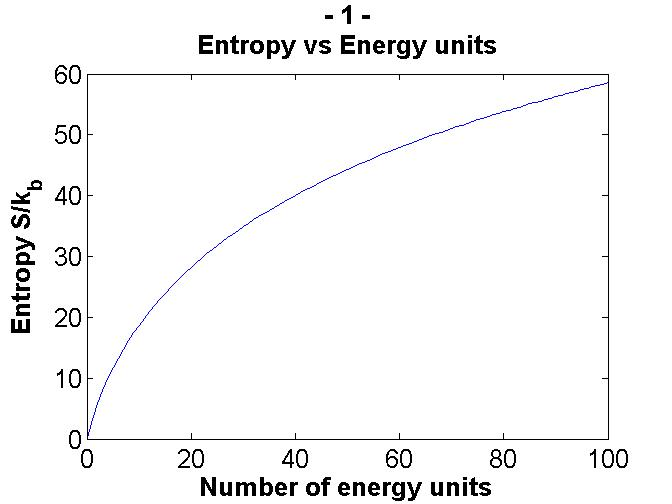
\includegraphics[width=0.45\textwidth]{P1.jpg}


\item \textbf{(10 pts)} 

The resulting temperature has units $\epsilon/k_\mathrm{b}$

\begin{verbatim}
U=q; %Energy in units of epsilon
T=diff(U)./diff(sok)
%Interpolate the vector U
Uint=(diff(U)*0.5+U(1:(end-1)))
\end{verbatim}

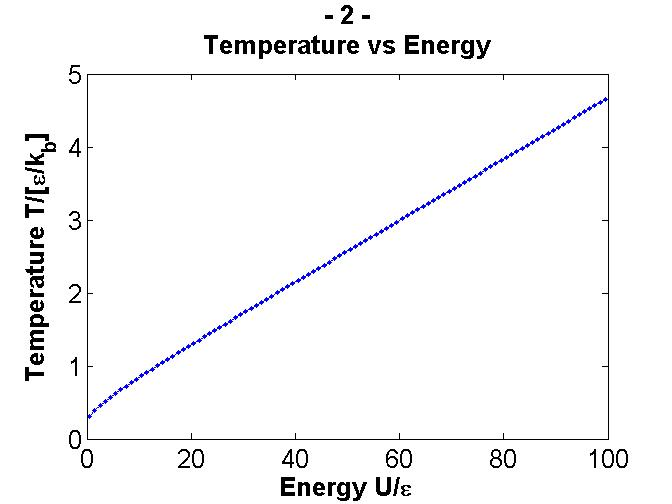
\includegraphics[width=0.45\textwidth]{P2.jpg}

\item \textbf{(10 pts)} 

\begin{verbatim}
%Interpolate the vector sok
sokint=(diff(sok)*0.5+sok(1:(end-1)))
\end{verbatim}

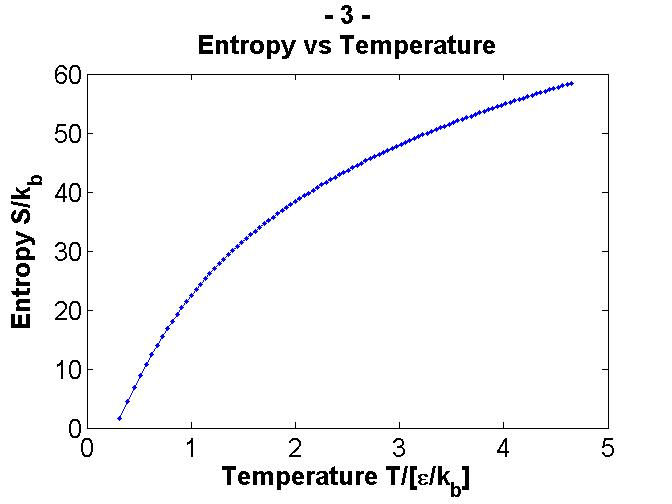
\includegraphics[width=0.45\textwidth]{P3.jpg}

\item \textbf{(20 pts)} 

The units of the heat capacity is just $k_\mathrm{b}$.

\begin{verbatim}
C=diff(Uint)./diff(T)
Tint=(diff(T)*0.5+T(1:(end-1)))
Uint2=(diff(Uint)*0.5+Uint(1:(end-1)))
\end{verbatim}

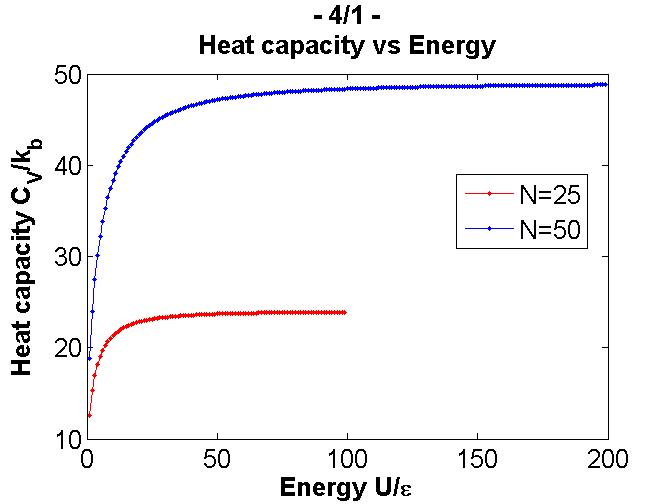
\includegraphics[width=0.45\textwidth]{P4_1.jpg}
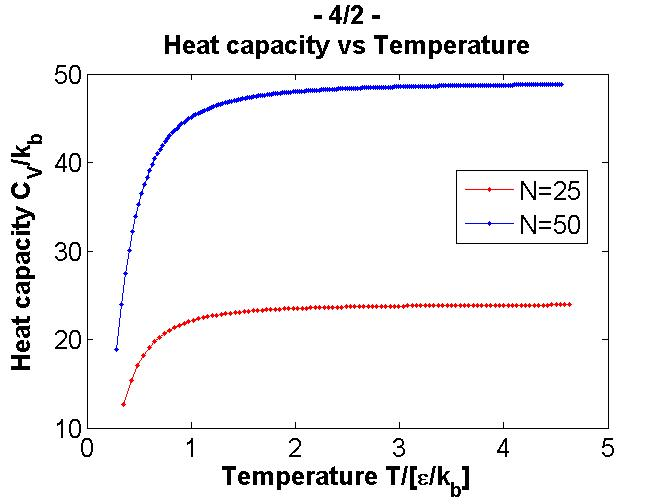
\includegraphics[width=0.45\textwidth]{P4_2.jpg}\\

A larger number of oscillators leads to a higher heat capacity. Larger number of oscillators $\rightarrow$ higher multiplicity and entropy $\rightarrow$ larger slope of the function S(U) $\rightarrow$ lower maximum temperature for a given energy range OR higher heat capacity $\rightarrow$ lower temperature for given internal energy OR any other explanation.

\end{enumerate}

\section*{Heat capacity of the Einstein solid  -- comparison to real examples (50 pts)}
\label{sec:lot}

\begin{enumerate}[resume]


\item \textbf{(15 pts)} 

\begin{verbatim}
clear all
clc

A_Pb=importdata('lead.dat');
C_Pb=A_Pb(:,2);
T_Pb=A_Pb(:,1);

A_Al=importdata('aluminum.dat');
C_Al=A_Al(:,2);
T_Al=A_Al(:,1);
\end{verbatim}

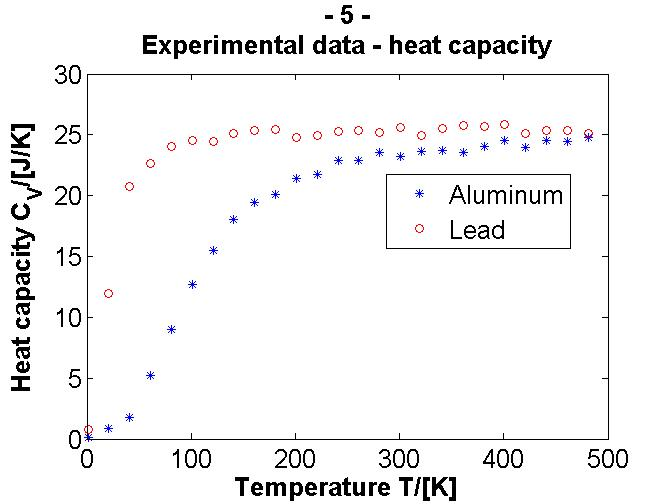
\includegraphics[width=0.45\textwidth]{P5.jpg}\\

\item \textbf{(20 pts)} 

\begin{verbatim}
T_exp=T_Pb;
C_exp=C_Pb;
%T_exp=T_Al;
%C_exp=C_Al;

Na=6.022*10^23;
kb=1.38*10^-23; %J/K
ev=1.6*10^-19;
C_func=@(eps) sum((C_exp-3*Na*kb.*(eps./(kb.*T_exp)).^2.*...
       exp(eps./(kb.*T_exp))./(exp(eps./(kb.*T_exp))-1).^2).^2)

epsf=fminsearch(C_func,0.01*ev)/ev
\end{verbatim}

$\epsilon_{Pb}=0{.}0055\,\mathrm{eV}$ 
$\epsilon_{Al}=0{.}0248\,\mathrm{eV}$ 


\item \textbf{(10 pts)} 

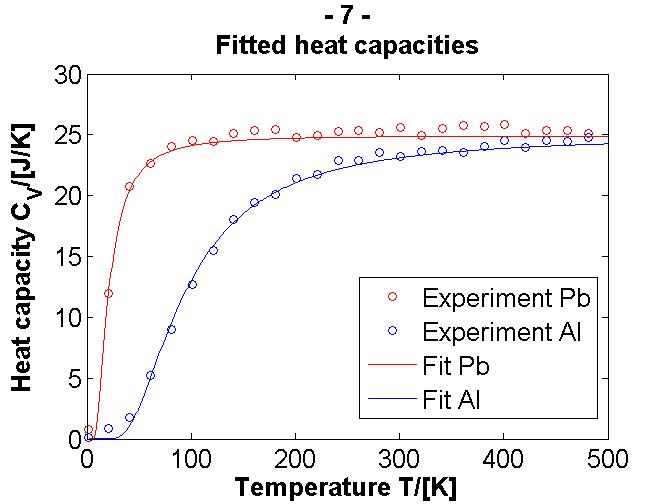
\includegraphics[width=0.45\textwidth]{P7.jpg}\\

\item \textbf{(5 pts)} 


The distance between the energy levels is proportional to the frequency $f$ of the oscillator $\epsilon=hf$. $h$ is Planck's constant. Therefore, higher values of $\epsilon$ are an indication for higher frequencies, higher spring constants, and therefore for stiffer/harder materials/higher speed of sound. 

\end{enumerate}


















\end{document}